%%=============================================================================
%% LaTeX sjabloon voor bachelorproef, HoGent Bedrijf en Organisatie
%% Opleiding Toegepaste Informatica
%%=============================================================================

\documentclass[fleqn,a4paper,12pt]{book}

%%=============================================================================
%% LaTeX sjabloon voor de bachelorproef, HoGent Bedrijf en Organisatie
%% Opleiding toegepaste informatica
%%
%% Structuur en algemene vormgeving. Meestal hoef je hier niets te wijzigen.
%%
%% Vormgeving gebaseerd op "The Legrand Orange Book", version 2.0 (9/2/15)
%% door Mathias Legrand (legrand.mathias@gmail.com) met aanpassingen door
%% Vel (vel@latextemplates.com). Het oorspronkelijke template is te vinden op
%% http://www.LaTeXTemplates.com
%%
%% Aanpassingen voor HoGent toegepaste informatica: 
%%   Bert Van Vreckem <bert.vanvreckem@hogent.be>
%% Licentie: 
%%   CC BY-NC-SA 3.0 (http://creativecommons.org/licenses/by-nc-sa/3.0/)
%%=============================================================================

%%-----------------------------------------------------------------------------
%% Packages
%%-----------------------------------------------------------------------------

\usepackage[top=3cm,bottom=3cm,left=3cm,right=3cm,headsep=10pt,a4paper]{geometry} % Page margins
\usepackage{wrapfig}
\usepackage[utf8]{inputenc}  % Accenten gebruiken in tekst (vb. é ipv \'e)
\usepackage{amsfonts}        % AMS math packages: extra wiskundige
\usepackage{amsmath}         %   symbolen (o.a. getallen-
\usepackage{amssymb}         %   verzamelingen N, R, Z, Q, etc.)
\usepackage[english,dutch]{babel}    % Taalinstellingen: woordsplitsingen,
                             %  commando's voor speciale karakters
                             %  ("dutch" voor NL)
\usepackage{iflang}
\usepackage{eurosym}         % Euro-symbool €
\usepackage{geometry}
\usepackage{graphicx}        % Invoegen van tekeningen
\graphicspath{{img/}}       % Specifies the directory where pictures are stored
\usepackage{tikz}            % Required for drawing custom shapes
\usepackage[pdftex,bookmarks=true]{hyperref}
                             % PDF krijgt klikbare links & verwijzingen,
                             %  inhoudstafel
\usepackage{enumitem}        % Customize lists
\setlist{nolistsep}         % Reduce spacing between list items
\usepackage{listings}        % Broncode mooi opmaken
\usepackage{multirow}        % Tekst over verschillende cellen in tabellen
\usepackage{rotating}        % Tabellen en figuren roteren

\usepackage{booktabs}        % Required for nicer horizontal rules in tables

\usepackage{xcolor}          % Required for specifying colors by name
\definecolor{maincolor}{RGB}{0,147,208} % Define the main color used for 
                             % highlighting throughout the book
                             % 0, 147, 208 = officiële kleur HoGent FBO

% Paragraph style: no indent, add space between paragraphs
\setlength{\parindent}{0em}
\setlength{\parskip}{1em}

\usepackage{etoolbox}
\usepackage{titling} % Macros for title, author, etc
\usepackage{lipsum}          % Voor vultekst (lorem ipsum)

%----------------------------------------------------------------------------------------
%	FONTS
%----------------------------------------------------------------------------------------

\usepackage{avant} % Use the Avantgarde font for headings
%\usepackage{times} % Use the Times font for headings
\usepackage{mathptmx} % Use the Adobe Times Roman as the default text font together with math symbols from the Sym­bol, Chancery and Com­puter Modern fonts

\usepackage{microtype} % Slightly tweak font spacing for aesthetics
\usepackage[utf8]{inputenc} % Required for including letters with accents
\usepackage[T1]{fontenc} % Use 8-bit encoding that has 256 glyphs

%------------------------------------------------------------------------------
%	TITLE PAGE
%------------------------------------------------------------------------------

\newcommand{\inserttitlepage}{%
\begin{titlepage}
  \newgeometry{top=2cm,bottom=1.5cm,left=1.5cm,right=1.5cm}
  \begin{center}

    \begingroup
    \rmfamily
    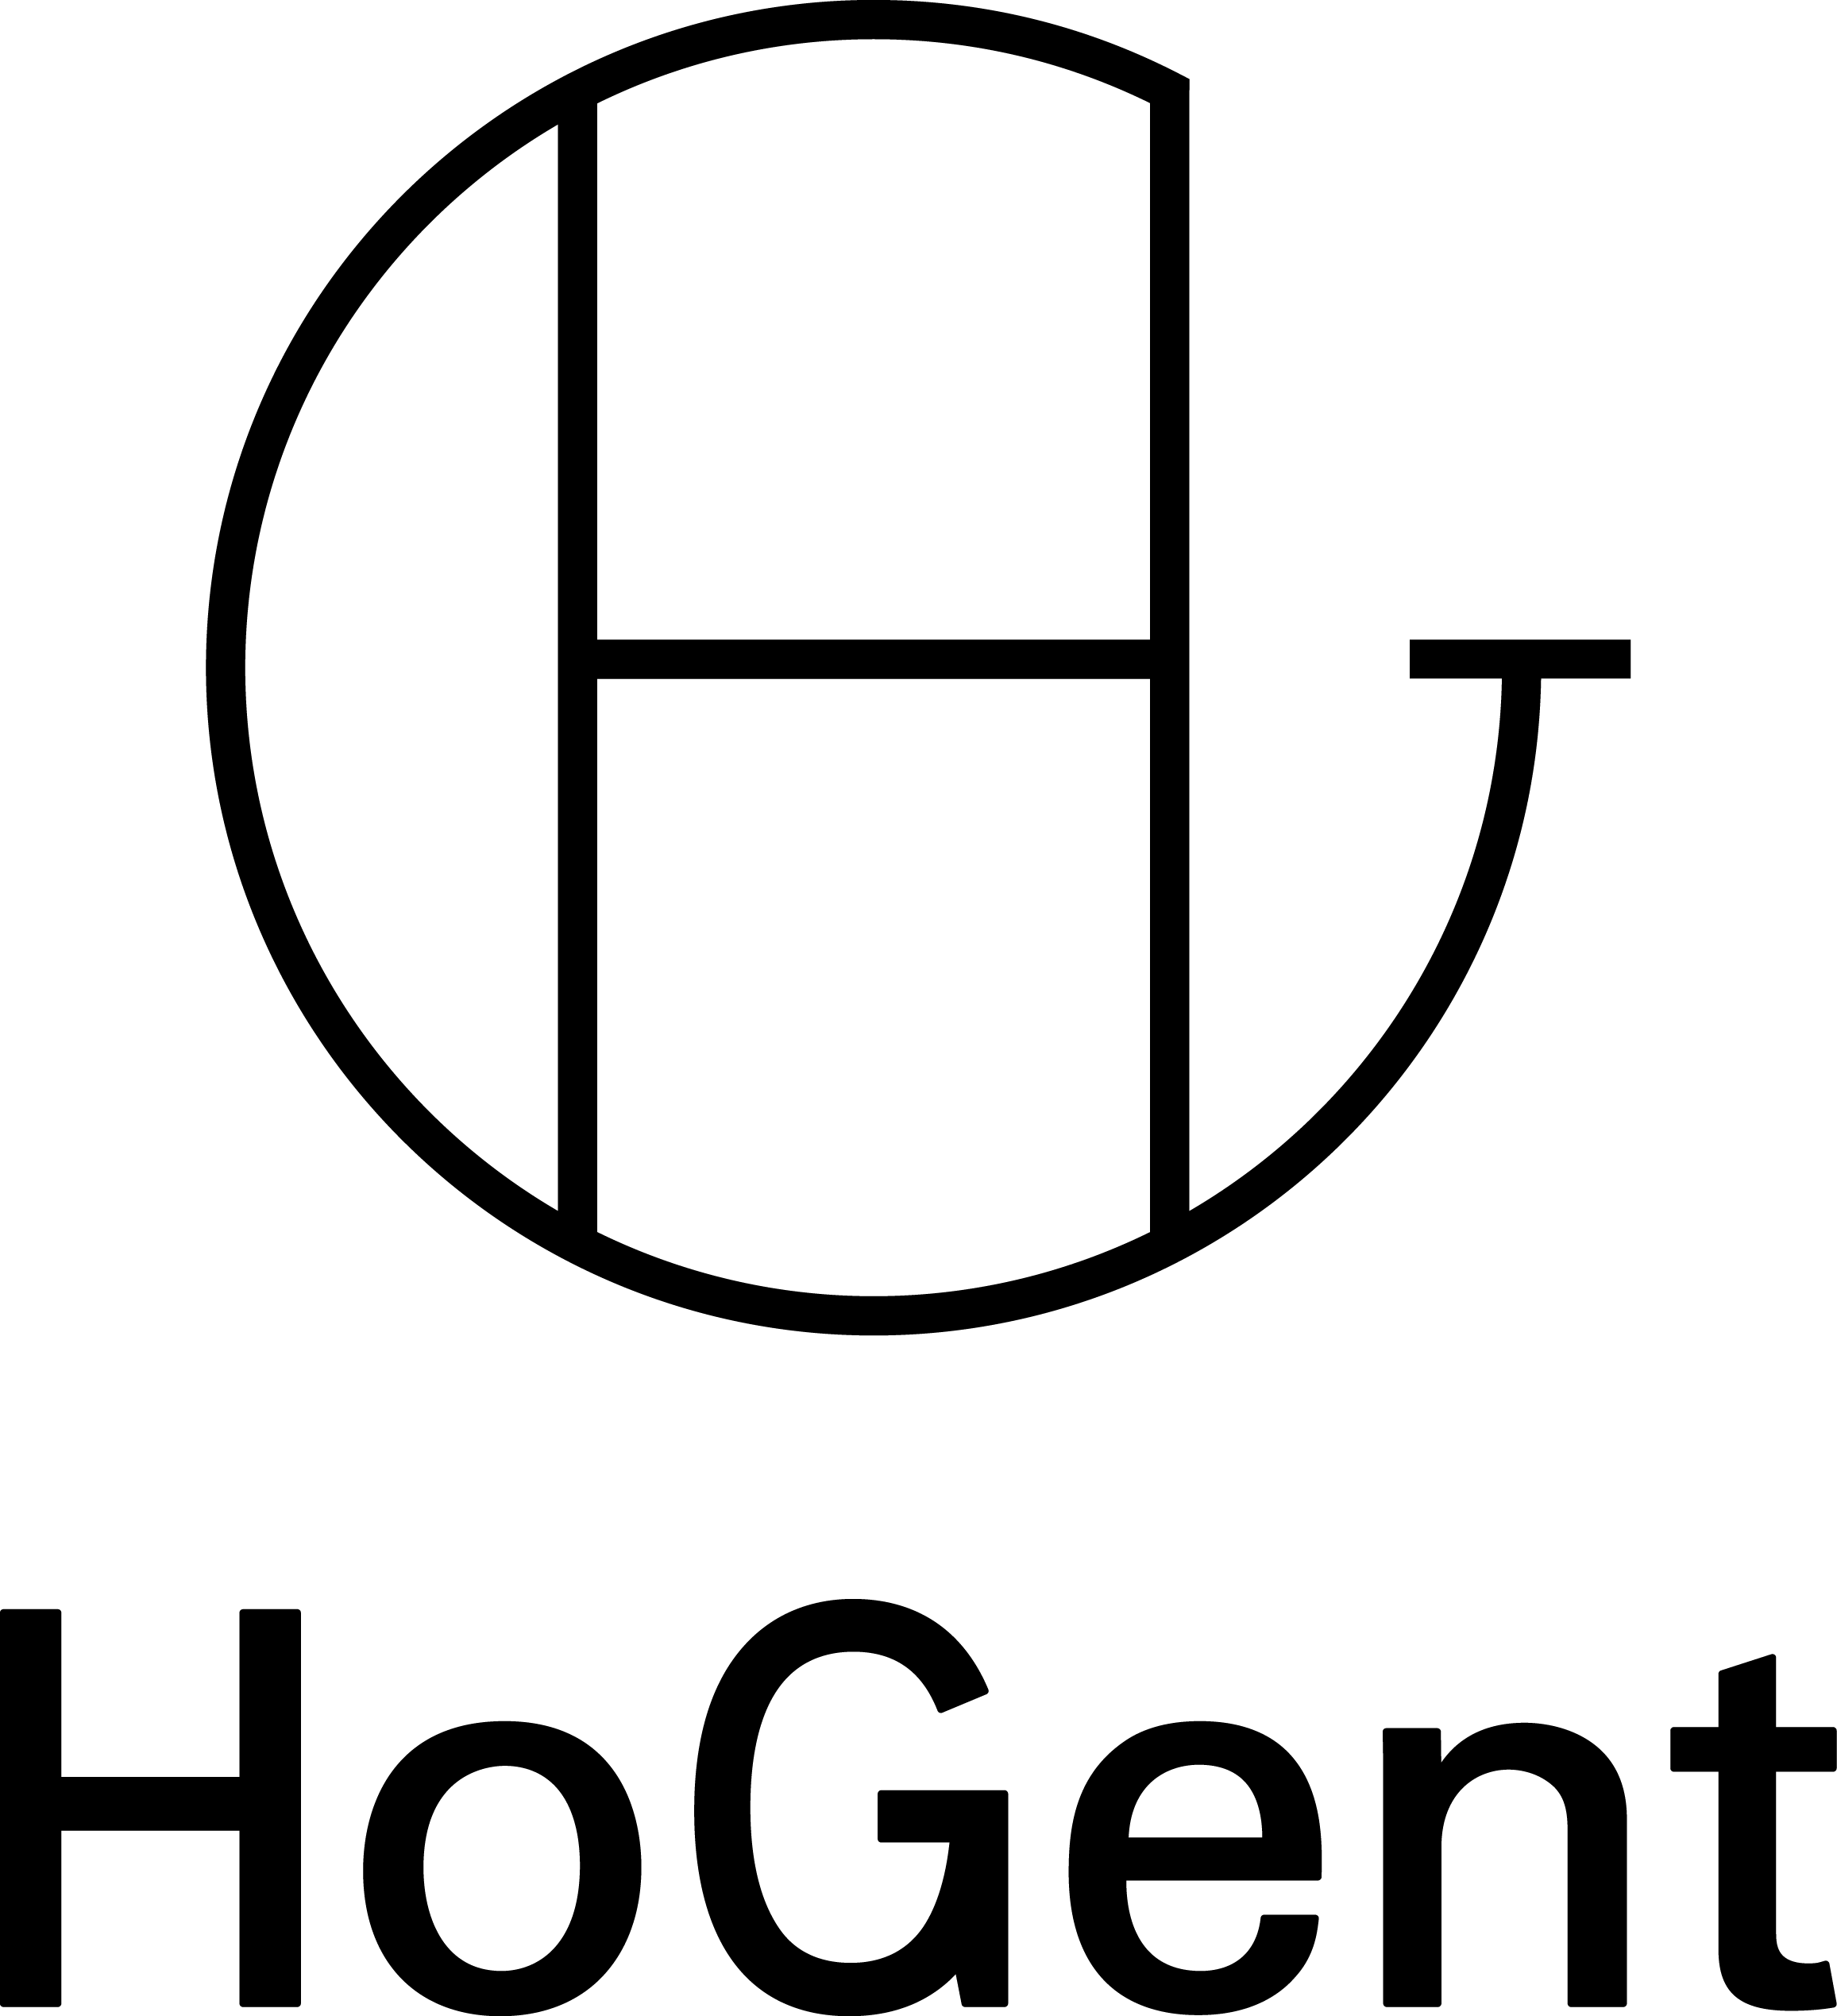
\includegraphics[width=2.5cm]{img/HG-beeldmerk-woordmerk}\\[.5cm]
    Faculteit Bedrijf en Organisatie\\[3cm]
    \titel
    \vfill
    \student\\[3.5cm]
    Scriptie voorgedragen tot het bekomen van de graad van\\professionele bachelor in de toegepaste informatica\\[2cm]
    Promotor:\\
    \promotor\\
    \ifdefempty{\copromotor}{\vspace{2.5cm}}{Co-promotor:\\\copromotor\\[2.5cm]}
    Instelling: \instelling\\[.5cm]
    Academiejaar: \academiejaar\\[.5cm]
    \ifcase \examenperiode \or Eerste \or Tweede \else Derde \fi examenperiode
    \endgroup

  \end{center}
  \restoregeometry
\end{titlepage}
  \emptypage
\begin{titlepage}
  \newgeometry{top=5.35cm,bottom=1.5cm,left=1.5cm,right=1.5cm}
  \begin{center}

    \begingroup
    \rmfamily
    \IfLanguageName{dutch}{Faculteit Bedrijf en Organisatie}{Faculty of Business and Information Management}\\[3cm]
    \titel
    \vfill
    \student\\[3.5cm]
    \IfLanguageName{dutch}{Scriptie voorgedragen tot het bekomen van de graad van\\professionele bachelor in de toegepaste informatica}{Thesis submitted in partial fulfilment of the requirements for the degree of\\professional bachelor of applied computer science}\\[2cm]
    Promotor:\\
    \promotor\\
    \ifdefempty{\copromotor}{\vspace{2.5cm}}{Co-promotor:\\\copromotor\\[2.5cm]}
    \IfLanguageName{dutch}{Instelling}{Institution}: \instelling\\[.5cm]
    \IfLanguageName{dutch}{Academiejaar}{Academic year}: \academiejaar\\[.5cm]
    \IfLanguageName{dutch}{%
    \ifcase \examenperiode \or Eerste \or Tweede \else Derde \fi examenperiode}{%
    \ifcase \examenperiode \or First \or Second \else Third \fi examination period}
    \endgroup

  \end{center}
  \restoregeometry
\end{titlepage}
}

%----------------------------------------------------------------------------------------
%	BIBLIOGRAPHY AND INDEX
%----------------------------------------------------------------------------------------

\usepackage[style=apa,backend=biber]{biblatex}
\usepackage{csquotes}
\DeclareLanguageMapping{dutch}{dutch-apa}
\addbibresource{bachproef-tin.bib} % BibTeX bibliography file
\addbibresource{../voorstel/voorstel.bib}
\defbibheading{bibempty}{}

\usepackage{calc} % For simpler calculation - used for spacing the index letter headings correctly
\usepackage{makeidx} % Required to make an index
\makeindex % Tells LaTeX to create the files required for indexing

%----------------------------------------------------------------------------------------
%	MAIN TABLE OF CONTENTS
%----------------------------------------------------------------------------------------

\usepackage{titletoc} % Required for manipulating the table of contents

\contentsmargin{0cm} % Removes the default margin

% Part text styling
\titlecontents{part}[0cm]
{\addvspace{20pt}\centering\large\bfseries}
{}
{}
{}

% Chapter text styling
\titlecontents{chapter}[1.25cm] % Indentation
{\addvspace{12pt}\large\sffamily\bfseries} % Spacing and font options for chapters
{\color{maincolor!60}\contentslabel[\Large\thecontentslabel]{1.25cm}\color{maincolor}} % Chapter number
{\color{maincolor}}
{\color{maincolor!60}\normalsize\;\titlerule*[.5pc]{.}\;\thecontentspage} % Page number

% Section text styling
\titlecontents{section}[1.25cm] % Indentation
{\addvspace{3pt}\sffamily\bfseries} % Spacing and font options for sections
{\contentslabel[\thecontentslabel]{1.25cm}} % Section number
{}
{\hfill\color{black}\thecontentspage} % Page number
[]

% Subsection text styling
\titlecontents{subsection}[1.25cm] % Indentation
{\addvspace{1pt}\sffamily\small} % Spacing and font options for subsections
{\contentslabel[\thecontentslabel]{1.25cm}} % Subsection number
{}
{\ \titlerule*[.5pc]{.}\;\thecontentspage} % Page number
[]

% List of figures
\titlecontents{figure}[0em]
{\addvspace{-5pt}\sffamily}
{\thecontentslabel\hspace*{1em}}
{}
{\ \titlerule*[.5pc]{.}\;\thecontentspage}
[]

% List of tables
\titlecontents{table}[0em]
{\addvspace{-5pt}\sffamily}
{\thecontentslabel\hspace*{1em}}
{}
{\ \titlerule*[.5pc]{.}\;\thecontentspage}
[]

%----------------------------------------------------------------------------------------
%	MINI TABLE OF CONTENTS IN PART HEADS
%----------------------------------------------------------------------------------------

% Chapter text styling
\titlecontents{lchapter}[0em] % Indenting
{\addvspace{15pt}\large\sffamily\bfseries} % Spacing and font options for chapters
{\color{maincolor}\contentslabel[\Large\thecontentslabel]{1.25cm}\color{maincolor}} % Chapter number
{}
{\color{maincolor}\normalsize\sffamily\bfseries\;\titlerule*[.5pc]{.}\;\thecontentspage} % Page number

% Section text styling
\titlecontents{lsection}[0em] % Indenting
{\sffamily\small} % Spacing and font options for sections
{\contentslabel[\thecontentslabel]{1.25cm}} % Section number
{}
{}

% Subsection text styling
\titlecontents{lsubsection}[.5em] % Indentation
{\normalfont\footnotesize\sffamily} % Font settings
{}
{}
{}

%----------------------------------------------------------------------------------------
%	PAGE HEADERS
%----------------------------------------------------------------------------------------

\usepackage{fancyhdr} % Required for header and footer configuration

\pagestyle{fancy}
\renewcommand{\chaptermark}[1]{\markboth{\sffamily\normalsize\bfseries\chaptername\ \thechapter.\ #1}{}} % Chapter text font settings
\renewcommand{\sectionmark}[1]{\markright{\sffamily\normalsize\thesection\hspace{5pt}#1}{}} % Section text font settings
\fancyhf{} \fancyhead[LE,RO]{\sffamily\normalsize\thepage} % Font setting for the page number in the header
\fancyhead[LO]{\rightmark} % Print the nearest section name on the left side of odd pages
\fancyhead[RE]{\leftmark} % Print the current chapter name on the right side of even pages
\renewcommand{\headrulewidth}{0.5pt} % Width of the rule under the header
\addtolength{\headheight}{2.5pt} % Increase the spacing around the header slightly
\renewcommand{\footrulewidth}{0pt} % Removes the rule in the footer
\fancypagestyle{plain}{\fancyhead{}\renewcommand{\headrulewidth}{0pt}} % Style for when a plain pagestyle is specified

% Removes the header from odd empty pages at the end of chapters
\makeatletter
\renewcommand{\cleardoublepage}{
\clearpage\ifodd\c@page\else
\hbox{}
\vspace*{\fill}
\thispagestyle{empty}
\newpage
\fi}

%----------------------------------------------------------------------------------------
%	THEOREM STYLES
%----------------------------------------------------------------------------------------

\usepackage{amsmath,amsfonts,amssymb,amsthm} % For math equations, theorems, symbols, etc

\newcommand{\intoo}[2]{\mathopen{]}#1\,;#2\mathclose{[}}
\newcommand{\ud}{\mathop{\mathrm{{}d}}\mathopen{}}
\newcommand{\intff}[2]{\mathopen{[}#1\,;#2\mathclose{]}}
\newtheorem{notation}{Notation}[chapter]

% Boxed/framed environments
\newtheoremstyle{maincolornumbox}% % Theorem style name
{0pt}% Space above
{0pt}% Space below
{\normalfont}% % Body font
{}% Indent amount
{\small\bf\sffamily\color{maincolor}}% % Theorem head font
{\;}% Punctuation after theorem head
{0.25em}% Space after theorem head
{\small\sffamily\color{maincolor}\thmname{#1}\nobreakspace\thmnumber{\@ifnotempty{#1}{}\@upn{#2}}% Theorem text (e.g. Theorem 2.1)
\thmnote{\nobreakspace\the\thm@notefont\sffamily\bfseries\color{black}---\nobreakspace#3.}} % Optional theorem note
\renewcommand{\qedsymbol}{$\blacksquare$}% Optional qed square

\newtheoremstyle{blacknumex}% Theorem style name
{5pt}% Space above
{5pt}% Space below
{\normalfont}% Body font
{} % Indent amount
{\small\bf\sffamily}% Theorem head font
{\;}% Punctuation after theorem head
{0.25em}% Space after theorem head
{\small\sffamily{\tiny\ensuremath{\blacksquare}}\nobreakspace\thmname{#1}\nobreakspace\thmnumber{\@ifnotempty{#1}{}\@upn{#2}}% Theorem text (e.g. Theorem 2.1)
\thmnote{\nobreakspace\the\thm@notefont\sffamily\bfseries---\nobreakspace#3.}}% Optional theorem note

\newtheoremstyle{blacknumbox} % Theorem style name
{0pt}% Space above
{0pt}% Space below
{\normalfont}% Body font
{}% Indent amount
{\small\bf\sffamily}% Theorem head font
{\;}% Punctuation after theorem head
{0.25em}% Space after theorem head
{\small\sffamily\thmname{#1}\nobreakspace\thmnumber{\@ifnotempty{#1}{}\@upn{#2}}% Theorem text (e.g. Theorem 2.1)
\thmnote{\nobreakspace\the\thm@notefont\sffamily\bfseries---\nobreakspace#3.}}% Optional theorem note

% Non-boxed/non-framed environments
\newtheoremstyle{maincolornum}% % Theorem style name
{5pt}% Space above
{5pt}% Space below
{\normalfont}% % Body font
{}% Indent amount
{\small\bf\sffamily\color{maincolor}}% % Theorem head font
{\;}% Punctuation after theorem head
{0.25em}% Space after theorem head
{\small\sffamily\color{maincolor}\thmname{#1}\nobreakspace\thmnumber{\@ifnotempty{#1}{}\@upn{#2}}% Theorem text (e.g. Theorem 2.1)
\thmnote{\nobreakspace\the\thm@notefont\sffamily\bfseries\color{black}---\nobreakspace#3.}} % Optional theorem note
\renewcommand{\qedsymbol}{$\blacksquare$}% Optional qed square
\makeatother

% Defines the theorem text style for each type of theorem to one of the three styles above
\newcounter{dummy}
\numberwithin{dummy}{section}
\theoremstyle{maincolornumbox}
\newtheorem{theoremeT}[dummy]{Theorem}
\newtheorem{problem}{Problem}[chapter]
\newtheorem{exerciseT}{Exercise}[chapter]
\theoremstyle{blacknumex}
\newtheorem{exampleT}{Example}[chapter]
\theoremstyle{blacknumbox}
\newtheorem{vocabulary}{Vocabulary}[chapter]
\newtheorem{definitionT}{Definition}[section]
\newtheorem{corollaryT}[dummy]{Corollary}
\theoremstyle{maincolornum}
\newtheorem{proposition}[dummy]{Proposition}

%----------------------------------------------------------------------------------------
%	DEFINITION OF COLORED BOXES
%----------------------------------------------------------------------------------------

\RequirePackage[framemethod=default]{mdframed} % Required for creating the theorem, definition, exercise and corollary boxes

% Theorem box
\newmdenv[skipabove=7pt,
skipbelow=7pt,
backgroundcolor=black!5,
linecolor=maincolor,
innerleftmargin=5pt,
innerrightmargin=5pt,
innertopmargin=5pt,
leftmargin=0cm,
rightmargin=0cm,
innerbottommargin=5pt]{tBox}

% Exercise box
\newmdenv[skipabove=7pt,
skipbelow=7pt,
rightline=false,
leftline=true,
topline=false,
bottomline=false,
backgroundcolor=maincolor!10,
linecolor=maincolor,
innerleftmargin=5pt,
innerrightmargin=5pt,
innertopmargin=5pt,
innerbottommargin=5pt,
leftmargin=0cm,
rightmargin=0cm,
linewidth=4pt]{eBox}

% Definition box
\newmdenv[skipabove=7pt,
skipbelow=7pt,
rightline=false,
leftline=true,
topline=false,
bottomline=false,
linecolor=maincolor,
innerleftmargin=5pt,
innerrightmargin=5pt,
innertopmargin=0pt,
leftmargin=0cm,
rightmargin=0cm,
linewidth=4pt,
innerbottommargin=0pt]{dBox}

% Corollary box
\newmdenv[skipabove=7pt,
skipbelow=7pt,
rightline=false,
leftline=true,
topline=false,
bottomline=false,
linecolor=gray,
backgroundcolor=black!5,
innerleftmargin=5pt,
innerrightmargin=5pt,
innertopmargin=5pt,
leftmargin=0cm,
rightmargin=0cm,
linewidth=4pt,
innerbottommargin=5pt]{cBox}

% Creates an environment for each type of theorem and assigns it a theorem text style from the "Theorem Styles" section above and a colored box from above
\newenvironment{theorem}{\begin{tBox}\begin{theoremeT}}{\end{theoremeT}\end{tBox}}
\newenvironment{exercise}{\begin{eBox}\begin{exerciseT}}{\hfill{\color{maincolor}\tiny\ensuremath{\blacksquare}}\end{exerciseT}\end{eBox}}
\newenvironment{definition}{\begin{dBox}\begin{definitionT}}{\end{definitionT}\end{dBox}}
\newenvironment{example}{\begin{exampleT}}{\hfill{\tiny\ensuremath{\blacksquare}}\end{exampleT}}
\newenvironment{corollary}{\begin{cBox}\begin{corollaryT}}{\end{corollaryT}\end{cBox}}

%----------------------------------------------------------------------------------------
%	REMARK ENVIRONMENT
%----------------------------------------------------------------------------------------

\newenvironment{remark}{\par\vspace{10pt}\small % Vertical white space above the remark and smaller font size
\begin{list}{}{
\leftmargin=35pt % Indentation on the left
\rightmargin=25pt}\item\ignorespaces % Indentation on the right
\makebox[-2.5pt]{\begin{tikzpicture}[overlay]
\node[draw=maincolor!60,line width=1pt,circle,fill=maincolor!25,font=\sffamily\bfseries,inner sep=2pt,outer sep=0pt] at (-15pt,0pt){\textcolor{maincolor}{R}};\end{tikzpicture}} % Orange R in a circle
\advance\baselineskip -1pt}{\end{list}\vskip5pt} % Tighter line spacing and white space after remark

%----------------------------------------------------------------------------------------
%	SECTION NUMBERING IN THE MARGIN
%----------------------------------------------------------------------------------------

\makeatletter
\renewcommand{\@seccntformat}[1]{\llap{\textcolor{maincolor}{\csname the#1\endcsname}\hspace{1em}}}
\renewcommand{\section}{\@startsection{section}{1}{\z@}
{-4ex \@plus -1ex \@minus -.4ex}
{1ex \@plus.2ex }
{\normalfont\large\sffamily\bfseries}}
\renewcommand{\subsection}{\@startsection {subsection}{2}{\z@}
{-3ex \@plus -0.1ex \@minus -.4ex}
{0.5ex \@plus.2ex }
{\normalfont\sffamily\bfseries}}
\renewcommand{\subsubsection}{\@startsection {subsubsection}{3}{\z@}
{-2ex \@plus -0.1ex \@minus -.2ex}
{.2ex \@plus.2ex }
{\normalfont\small\sffamily\bfseries}}
\renewcommand\paragraph{\@startsection{paragraph}{4}{\z@}
{-2ex \@plus-.2ex \@minus .2ex}
{.1ex}
{\normalfont\small\sffamily\bfseries}}

%----------------------------------------------------------------------------------------
%	PART HEADINGS
%----------------------------------------------------------------------------------------

% numbered part in the table of contents
\newcommand{\@mypartnumtocformat}[2]{%
\setlength\fboxsep{0pt}%
\noindent\colorbox{maincolor!20}{\strut\parbox[c][.7cm]{\ecart}{\color{maincolor!70}\Large\sffamily\bfseries\centering#1}}\hskip\esp\colorbox{maincolor!40}{\strut\parbox[c][.7cm]{\linewidth-\ecart-\esp}{\Large\sffamily\centering#2}}}%
%%%%%%%%%%%%%%%%%%%%%%%%%%%%%%%%%%
% unnumbered part in the table of contents
\newcommand{\@myparttocformat}[1]{%
\setlength\fboxsep{0pt}%
\noindent\colorbox{maincolor!40}{\strut\parbox[c][.7cm]{\linewidth}{\Large\sffamily\centering#1}}}%
%%%%%%%%%%%%%%%%%%%%%%%%%%%%%%%%%%
\newlength\esp
\setlength\esp{4pt}
\newlength\ecart
\setlength\ecart{1.2cm-\esp}
\newcommand{\thepartimage}{}%
\newcommand{\partimage}[1]{\renewcommand{\thepartimage}{#1}}%
\def\@part[#1]#2{%
\ifnum \c@secnumdepth >-2\relax%
\refstepcounter{part}%
\addcontentsline{toc}{part}{\texorpdfstring{\protect\@mypartnumtocformat{\thepart}{#1}}{\partname~\thepart\ ---\ #1}}
\else%
\addcontentsline{toc}{part}{\texorpdfstring{\protect\@myparttocformat{#1}}{#1}}%
\fi%
\startcontents%
\markboth{}{}%
{\thispagestyle{empty}%
\begin{tikzpicture}[remember picture,overlay]%
\node at (current page.north west){\begin{tikzpicture}[remember picture,overlay]%
\fill[maincolor!20](0cm,0cm) rectangle (\paperwidth,-\paperheight);
\node[anchor=north] at (4cm,-3.25cm){\color{maincolor!40}\fontsize{220}{100}\sffamily\bfseries\@Roman\c@part};
\node[anchor=south east] at (\paperwidth-1cm,-\paperheight+1cm){\parbox[t][][t]{8.5cm}{
\printcontents{l}{0}{\setcounter{tocdepth}{1}}%
}};
\node[anchor=north east] at (\paperwidth-1.5cm,-3.25cm){\parbox[t][][t]{15cm}{\strut\raggedleft\color{white}\fontsize{30}{30}\sffamily\bfseries#2}};
\end{tikzpicture}};
\end{tikzpicture}}%
\@endpart}
\def\@spart#1{%
\startcontents%
\phantomsection
{\thispagestyle{empty}%
\begin{tikzpicture}[remember picture,overlay]%
\node at (current page.north west){\begin{tikzpicture}[remember picture,overlay]%
\fill[maincolor!20](0cm,0cm) rectangle (\paperwidth,-\paperheight);
\node[anchor=north east] at (\paperwidth-1.5cm,-3.25cm){\parbox[t][][t]{15cm}{\strut\raggedleft\color{white}\fontsize{30}{30}\sffamily\bfseries#1}};
\end{tikzpicture}};
\end{tikzpicture}}
\addcontentsline{toc}{part}{\texorpdfstring{%
\setlength\fboxsep{0pt}%
\noindent\protect\colorbox{maincolor!40}{\strut\protect\parbox[c][.7cm]{\linewidth}{\Large\sffamily\protect\centering #1\quad\mbox{}}}}{#1}}%
\@endpart}
\def\@endpart{\vfil\newpage
\if@twoside
\if@openright
\null
\thispagestyle{empty}%
\newpage
\fi
\fi
\if@tempswa
\twocolumn
\fi}

%----------------------------------------------------------------------------------------
%	CHAPTER HEADINGS
%----------------------------------------------------------------------------------------

% A switch to conditionally include a picture, implemented by  Christian Hupfer
\newif\ifusechapterimage
\usechapterimagetrue
\newcommand{\thechapterimage}{}%
\newcommand{\chapterimage}[1]{\ifusechapterimage\renewcommand{\thechapterimage}{#1}\fi}%
\def\@makechapterhead#1{%
{\parindent \z@ \raggedright \normalfont
\ifnum \c@secnumdepth >\m@ne
\if@mainmatter
\begin{tikzpicture}[remember picture,overlay]
\node at (current page.north west)
{\begin{tikzpicture}[remember picture,overlay]
\node[anchor=north west,inner sep=0pt] at (0,0) {\ifusechapterimage\includegraphics[width=\paperwidth]{\thechapterimage}\fi};
\draw[anchor=west] (\Gm@lmargin,-9cm) node [line width=2pt,rounded corners=15pt,draw=maincolor,fill=white,fill opacity=0.5,inner sep=15pt]{\strut\makebox[22cm]{}};
\draw[anchor=west] (\Gm@lmargin+.3cm,-9cm) node {\huge\sffamily\bfseries\color{black}\thechapter. #1\strut};
\end{tikzpicture}};
\end{tikzpicture}
\else
\begin{tikzpicture}[remember picture,overlay]
\node at (current page.north west)
{\begin{tikzpicture}[remember picture,overlay]
\node[anchor=north west,inner sep=0pt] at (0,0) {\ifusechapterimage\includegraphics[width=\paperwidth]{\thechapterimage}\fi};
\draw[anchor=west] (\Gm@lmargin,-9cm) node [line width=2pt,rounded corners=15pt,draw=maincolor,fill=white,fill opacity=0.5,inner sep=15pt]{\strut\makebox[22cm]{}};
\draw[anchor=west] (\Gm@lmargin+.3cm,-9cm) node {\huge\sffamily\bfseries\color{black}#1\strut};
\end{tikzpicture}};
\end{tikzpicture}
\fi\fi\par\vspace*{270\p@}}}

%-------------------------------------------

\def\@makeschapterhead#1{%
\begin{tikzpicture}[remember picture,overlay]
\node at (current page.north west)
{\begin{tikzpicture}[remember picture,overlay]
\node[anchor=north west,inner sep=0pt] at (0,0) {\ifusechapterimage\includegraphics[width=\paperwidth]{\thechapterimage}\fi};
\draw[anchor=west] (\Gm@lmargin,-9cm) node [line width=2pt,rounded corners=15pt,draw=maincolor,fill=white,fill opacity=0.5,inner sep=15pt]{\strut\makebox[22cm]{}};
\draw[anchor=west] (\Gm@lmargin+.3cm,-9cm) node {\huge\sffamily\bfseries\color{black}#1\strut};
\end{tikzpicture}};
\end{tikzpicture}
\par\vspace*{270\p@}}
\makeatother

%----------------------------------------------------------------------------------------
%	HYPERLINKS IN THE DOCUMENTS
%----------------------------------------------------------------------------------------

\usepackage{hyperref}
\hypersetup{hidelinks,backref=true,pagebackref=true,hyperindex=true,colorlinks=false,breaklinks=true,urlcolor= maincolor,bookmarks=true,bookmarksopen=false,pdftitle={Title},pdfauthor={Author}}
\usepackage{bookmark}
\bookmarksetup{
open,
numbered,
addtohook={%
\ifnum\bookmarkget{level}=0 % chapter
\bookmarksetup{bold}%
\fi
\ifnum\bookmarkget{level}=-1 % part
\bookmarksetup{color=maincolor,bold}%
\fi
}
}

%----------------------------------------------------------------------------------------
%	Java source code
%----------------------------------------------------------------------------------------

% Commando voor invoegen Java-broncodebestanden (dank aan Niels Corneille)
% Gebruik:
%   \codefragment{source/MijnKlasse.java}{Uitleg bij de code}
%
% Je kan dit aanpassen aan de taal die je zelf het meeste gebruikt in je
% bachelorproef.
\newcommand{\codefragment}[2]{ \lstset{%
  language=java,
  breaklines=true,
  float=th,
  caption={#2},
  basicstyle=\scriptsize,
  frame=single,
  extendedchars=\true
}
\lstinputlisting{#1}}

% Leeg blad
\newcommand{\emptypage}{%
\newpage
\thispagestyle{empty}
\mbox{}
\newpage
}


%%---------- Documenteigenschappen --------------------------------------------
%% TODO: Vul dit aan met je eigen info:

% Je eigen naam
\newcommand{\student}{Dylan Van Paemel}

% De naam van je promotor (lector van de opleiding)
\newcommand{\promotor}{Noemie Slaats}

% De naam van je co-promotor. Als je promotor ook je opdrachtgever is en je
% dus ook inhoudelijk begeleidt (en enkel dan!), mag je dit leeg laten.
\newcommand{\copromotor}{Wouter Van Peteghem}

% Indien je bachelorproef in opdracht van/in samenwerking met een bedrijf of
% externe organisatie geschreven is, geef je hier de naam. Zoniet laat je dit
% zoals het is.
\newcommand{\instelling}{---}

% De titel van het rapport/bachelorproef
\newcommand{\titel}{Titel}

% Datum van indienen (gebruik telkens de deadline, ook al geef je eerder af)
\newcommand{\datum}{11 jan 2019}

% Academiejaar
\newcommand{\academiejaar}{2018-2019}
% Examenperiode
%  - 1e semester = 1e examenperiode => 1
%  - 2e semester = 2e examenperiode => 2
%  - tweede zit  = 3e examenperiode => 3
\newcommand{\examenperiode}{1}
%%=============================================================================
%% Inhoud document
%%=============================================================================

\begin{document}

%---------- Taalselectie ------------------------------------------------------
% Als je je bachelorproef in het Engels schrijft, haal dan onderstaande regel
% uit commentaar. Let op: de tekst op de voorkaft blijft in het Nederlands, en
% dat is ook de bedoeling!

%\selectlanguage{english}

%---------- Titelblad ---------------------------------------------------------
\inserttitlepage

%---------- Samenvatting, voorwoord -------------------------------------------
\usechapterimagefalse
%%=============================================================================
%% Voorwoord
%%=============================================================================

\chapter*{Woord vooraf}
\label{ch:voorwoord}

%% TODO:
%% Het voorwoord is het enige deel van de bachelorproef waar je vanuit je
%% eigen standpunt (``ik-vorm'') mag schrijven. Je kan hier bv. motiveren
%% waarom jij het onderwerp wil bespreken.
%% Vergeet ook niet te bedanken wie je geholpen/gesteund/... heeft



%%=============================================================================
%% Samenvatting
%%=============================================================================

% TODO: De "abstract" of samenvatting is een kernachtige (~ 1 blz. voor een
% thesis) synthese van het document.
%
% Deze aspecten moeten zeker aan bod komen:
% - Context: waarom is dit werk belangrijk?
% - Nood: waarom moest dit onderzocht worden?
% - Taak: wat heb je precies gedaan?
% - Object: wat staat in dit document geschreven?
% - Resultaat: wat was het resultaat?
% - Conclusie: wat is/zijn de belangrijkste conclusie(s)?
% - Perspectief: blijven er nog vragen open die in de toekomst nog kunnen
%    onderzocht worden? Wat is een mogelijk vervolg voor jouw onderzoek?
%
% LET OP! Een samenvatting is GEEN voorwoord!

%%---------- Nederlandse samenvatting -----------------------------------------
%
% TODO: Als je je bachelorproef in het Engels schrijft, moet je eerst een
% Nederlandse samenvatting invoegen. Haal daarvoor onderstaande code uit
% commentaar.
% Wie zijn bachelorproef in het Nederlands schrijft, kan dit negeren, de inhoud
% wordt niet in het document ingevoegd.

\IfLanguageName{english}{%
\selectlanguage{dutch}
\chapter*{Samenvatting}
\lipsum[1-4]
\selectlanguage{english}
}{}

%%---------- Samenvatting -----------------------------------------------------
% De samenvatting in de hoofdtaal van het document

\chapter*{\IfLanguageName{dutch}{Samenvatting}{Abstract}}

\lipsum[1-4]



%---------- Inhoudstafel ------------------------------------------------------
\pagestyle{empty} % No headers
\tableofcontents % Print the table of contents itself
\cleardoublepage % Forces the first chapter to start on an odd page so it's on the right
\pagestyle{fancy} % Print headers again

%---------- Lijst figuren, afkortingen, ... -----------------------------------

% Indien gewenst kan je hier een lijst van figuren/tabellen opgeven. Geef in
% dat geval je figuren/tabellen altijd een korte beschrijving:
%
%  \caption[korte beschrijving]{uitgebreide beschrijving}

\listoffigures
\listoftables

% Als je een lijst van afkortingen of termen wil toevoegen, dan hoort die
% hier thuis. Gebruik bijvoorbeeld de ``glossaries'' package.
% https://www.sharelatex.com/learn/Glossaries

%%---------- Kern -------------------------------------------------------------

%%=============================================================================
%% Inleiding
%%=============================================================================

\chapter{Inleiding}
\label{ch:inleiding}

De inleiding moet de lezer net genoeg informatie verschaffen om het onderwerp te begrijpen en in te zien waarom de onderzoeksvraag de moeite waard is om te onderzoeken. In de inleiding ga je literatuurverwijzingen beperken, zodat de tekst vlot leesbaar blijft. Je kan de inleiding verder onderverdelen in secties als dit de tekst verduidelijkt. Zaken die aan bod kunnen komen in de inleiding~\autocite{Pollefliet2011}:

\begin{itemize}
  \item context, achtergrond
  \item afbakenen van het onderwerp
  \item verantwoording van het onderwerp, methodologie
  \item probleemstelling
  \item onderzoeksdoelstelling
  \item onderzoeksvraag
  \item \ldots
\end{itemize}

\section{Probleemstelling}
\label{sec:probleemstelling}

Uit je probleemstelling moet duidelijk zijn dat je onderzoek een meerwaarde heeft voor een concrete doelgroep. De doelgroep moet goed gedefinieerd en afgelijnd zijn. Doelgroepen als ``bedrijven,'' ``KMO's,'' systeembeheerders, enz.~zijn nog te vaag. Als je een lijstje kan maken van de personen/organisaties die een meerwaarde zullen vinden in deze bachelorproef (dit is eigenlijk je steekproefkader), dan is dat een indicatie dat de doelgroep goed gedefinieerd is. Dit kan een enkel bedrijf zijn of zelfs één persoon (je co-promotor/opdrachtgever).

\section{Onderzoeksvraag}
\label{sec:onderzoeksvraag}

Wees zo concreet mogelijk bij het formuleren van je onderzoeksvraag. Een onderzoeksvraag is trouwens iets waar nog niemand op dit moment een antwoord heeft (voor zover je kan nagaan). Het opzoeken van bestaande informatie (bv. ``welke tools bestaan er voor deze toepassing?'') is dus geen onderzoeksvraag. Je kan de onderzoeksvraag verder specifiëren in deelvragen. Bv.~als je onderzoek gaat over performantiemetingen, dan 

\section{Onderzoeksdoelstelling}
\label{sec:onderzoeksdoelstelling}

Wat is het beoogde resultaat van je bachelorproef? Wat zijn de criteria voor succes? Beschrijf die zo concreet mogelijk.

\section{Opzet van deze bachelorproef}
\label{sec:opzet-bachelorproef}

% Het is gebruikelijk aan het einde van de inleiding een overzicht te
% geven van de opbouw van de rest van de tekst. Deze sectie bevat al een aanzet
% die je kan aanvullen/aanpassen in functie van je eigen tekst.

De rest van deze bachelorproef is als volgt opgebouwd:

In Hoofdstuk~\ref{ch:stand-van-zaken} wordt een overzicht gegeven van de stand van zaken binnen het onderzoeksdomein, op basis van een literatuurstudie.

In Hoofdstuk~\ref{ch:methodologie} wordt de methodologie toegelicht en worden de gebruikte onderzoekstechnieken besproken om een antwoord te kunnen formuleren op de onderzoeksvragen.

% TODO: Vul hier aan voor je eigen hoofstukken, één of twee zinnen per hoofdstuk

In Hoofdstuk~\ref{ch:conclusie}, tenslotte, wordt de conclusie gegeven en een antwoord geformuleerd op de onderzoeksvragen. Daarbij wordt ook een aanzet gegeven voor toekomstig onderzoek binnen dit domein.


\chapter{Literatuurstudie}
\label{ch:literatuurstudie}

% Tip: Begin elk hoofdstuk met een paragraaf inleiding die beschrijft hoe
% dit hoofdstuk past binnen het geheel van de bachelorproef. Geef in het
% bijzonder aan wat de link is met het vorige en volgende hoofdstuk.

% Pas na deze inleidende paragraaf komt de eerste sectiehoofding.

In dit hoofdstuk wordt er meer achtergrondinformatie gegeven. Het hoofdstuk start met extra informatie over mobile coaching apps. Daarna worden onderzoeken die in het verleden zijn gedaan naar mobile coaching bestudeerd. 

\section{Stand van zaken in het onderzoeksdomein}
\label{sec:stand-van-zaken}

Door de grote opkomst van smartphones, zijn er al enkele onderzoeken gedaan naar gezondheidsapplicaties. Deze studies stellen de kwaliteit van de applicaties in vraag. In de onderzoeken gaan ze na of het gebruik van dergelijke apps wel een positief effect heeft op de gezondheid van de mensen. 

Er zijn ook onderzoeken in dit domein die de evolutie van gezondheidsapplicaties bestuderen en bekijken hoe we in de toekomst nog betere applicaties kunnen maken. In 2013 ~\autocite{Wikipedia2013} was er een nieuwe trend, namelijk de smartwatch. Vanaf dan ging deze markt in een stroomversnelling en werd integratie met applicaties mogelijk. Applicatie ontwikkelaars hadden dus een nieuwe functie om als eerste op in te spelen. 
\newpage

\section{Werking van mobile coaching applicaties}
\label{sec:werking}

Mobile coaching applicaties werken praktisch altijd op dezelfde manier. Een gebruiker of een apparaat ( bv. Een smartwatch) levert input  zoals aantal stappen, aantal uren slaap, hartslagfrequentie, gepresteerde oefening of gegeten voeding. De applicatie kan verder aan de slag met de data te verwerken. Sommige van deze applicaties hebben ook een extra functie waardoor je externe apps kunt koppelen aan jouw coaching applicatie. Bijvoorbeeld kan Myfitnesspal gekoppeld worden met stappentellers en trainingsapplicaties. De calorieteller houdt dan rekening met de beweging van de gebruiker die dag en deze calorieën worden dan in vermindering gebracht. 

Stappentellers zijn hier een uitstekend voorbeeld van. Maar over het algemeen dient de gebruiker zelf aan de applicatie te vertellen wat hij of zij gedaan heeft. Het is afhankelijk van applicatie tot applicatie wat je precies allemaal kunt invoeren. 

De data wordt meestal in de cloud opgeslagen zodat deze toegankelijk wordt op alle toestellen van de gebruiker. Zo kan de gebruiker ook z’n resultaten bekijken op de computer door zich aan te melden op het online platform.

Mobile coaching applicaties komen volledig tot hun recht als gebruikers alle gegevens elke dag of trainingsdag bijhouden in de app. Dan kan de gebruiker na verloop van tijd z’n eigen progressie zien en analyses maken op de data van het verleden.

In onderstaande afbeelding wordt de algemene werking van een mobile coaching applicatie geïllustreerd. De gebruiker draagt een smartwatch die input levert samen met de smartphone. 

De data wordt allemaal gesynchroniseerd in de cloud zodat dit op elk moment kan opgevraagd worden door een ander apparaat die ook verbonden is met het account van de gebruiker

\begin{figure}[h!]
\centering
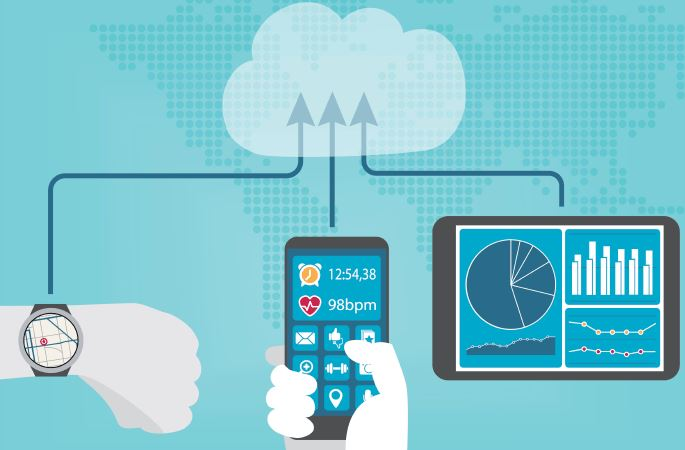
\includegraphics[width=0.7\textwidth]{img/cloud-synch.JPG}
\caption{werking mobile coaching apps (patientengagementhit.com,2017)}
\end{figure}

\newpage
\section{Verschillende types mobile coaching applicaties}
\label{sec:types}

Er zijn verschillende types mobile coaching applicaties waaruit je kan kiezen. In dit onderzoek is gekozen om de volgende 3 rubrieken te onderzoeken omdat er tussen deze types een significant verschil is:

\begin{itemize}
\setlength\itemsep{1em}
\item {\bf Voedingsapplicaties:} Deze applicaties begeleiden gebruikers alleen op het vlak van dieet en voeding. Dergelijke apps werken met een puntensysteem of met calorieën zodat gebruikers ofwel gewicht kunnen aankomen of afvallen, dit is natuurlijk afhankelijk van het doel van de gebruikers.

\item {\bf Trainingsapplicaties:} leiden tot schema’s die gebruikers zullen volgen bij hun training. Het schema zal vooraf worden ingesteld met het doel van de gebruiker bijvoorbeeld intensiteit of niveau van de oefeningen op het trainingsschema.

\item {\bf Coaching applicaties:} steunen de gebruikers door de dag heen grotendeels op gebied van training. Daarbij zal dit type applicaties ook fungeren als een virtuele coach die je nog extra motiveert om te bewegen. Als je niet aan je dagelijkse behoefte zit, dan zul je meldingen op je smartphone ontvangen enzovoort. Deze applicaties focussen zich niet alleen fysisch maar ook mentaal. Deze apps dienen als centraal punt voor alle andere bewegingsapps, ze verzamelen zoveel mogelijk data om de gebruiker zo efficiënt mogelijk te helpen.

\end{itemize}

\section{Vergelijkbare onderzoeken}
\label{sec:vergelijkbare-onderzoeken}

In dit onderdeel zullen vergelijkbare onderzoeken toegelicht worden. Er zal telkens een korte inhoud geschetst worden. 

\subsection{Hoe maak je betere fitness applicaties}
\label{sec:betere-apps}

Eerst wordt een artikel van The App Solutions \autocite{TheAppSolutions2017} bekeken die algemeen beschrijft hoe een ideale fitness app is opgebouwd. Zij verdelen de applicaties in 3 categorieën. Deze 3 categorieën zijn ook gekozen in dit onderzoek. De beschrijvingen van alle categorieën zijn ter verduidelijking.

\begin{itemize}
\setlength\itemsep{1em}
\item {\bf Dieet – en voedingsapplicaties:  } helpen gebruikers om zicht te krijgen op hun eetpatroon. Meestal maken dergelijk applicaties gebruik van calorieën. De gebruiker geeft zelf in wat er per maaltijd gegeten wordt. De applicatie herkent het product meestal en berekent zo de calorieën. Gebruikers stellen zelf hun limiet in door een doel te selecteren ( bijvoorbeeld ‘afvallen’) en de applicatie zegt hoeveel je mag en kan eten om het doel te bereiken.

Gegeven tips voor dit type: Het integreren van een boodschappenlijstje met suggesties voor recepten. Zo kunnen gebruikers makkelijker inschattingen maken. Bovendien helpen ze ook bij het maken van keuzes in de supermarkt. Het voorzien van een barcode scanner zodat gebruikers makkelijk hun voeding kunnen terugvinden in de database van de applicatie. Het versnelt ook het proces waardoor gebruikers minder moeite moeten doen om hun etenswaren te vinden.

\item {\bf Apps die gebruikt worden als activiteiten logboek (Mobile coaching) : } De applicaties kunnen zowel automatisch fysische activiteiten registreren door sensors in smartphones of als de gebruiker manueel zijn activiteit ingeeft. Dit type applicaties is handig om vooruitgang te zien omdat ze de mogelijkheid bieden om grafieken te genereren van prestaties in het verleden.

Gegeven tips voor dit type: Voor de gebruikers is het praktischer om een account te kunnen aanmaken omdat ze op die manier de mogelijkheid krijgen om de prestaties op andere toestellen te bekijken zoals tablet of computer. Tegenwoordig heeft bijna iedere sporter een smartwatch dus het is handig om deze te integreren in de applicatie, hierdoor moeten gebruikers ook zelf minder data manueel ingeven. Sociale media is een populair middeltje om gebruikers hun prestaties te laten delen met de buitenwereld. Het zorgt overigens voor publiciteit van de gebruikte applicatie en het kan dienen als extra motivatie voor de gebruiker als ze steun krijgen van vrienden. Geolocatie bepaalt de positie van de gebruiker door middel van een GPS-signaal. Daardoor kunnen gebruikers routes terug bekijken als ze dat wensen. Een laatste tip zijn push noticataties. Deze notificaties verschijnen als melding op het hoofdscherm van de smartphone. Ze zorgen ervoor dat gebruikers worden aangemoedigd en herinnerd om te bewegen.
\item {\bf  Fitness applicaties:  } Deze applicaties zorgen ervoor dat gebruikers makkelijker een eigen trainingsschema kunnen samenstellen. Als gebruikers de applicatie voor het eerst opstarten dan doorloopt de applicatie een aantal vragen en op basis van het antwoord wordt dan een trainingsschema gegenereerd.
Gegevens tips voor dit type zijn niet gespecifieerd in dit artikel. Meest van bovenstaande tips zijn hier ook van toepassing. 
\end{itemize}

\subsection{Onderzoek naar kwaliteit van mobile coaching applicaties met ACSM-richtlijnen}
\label{sec:onderzoek-ACSM-richtlijnen}

In het artikel van University of Florida \autocite{mhealth2015} bestuderen ze de kwaliteit van mobile coaching applicaties die op dat moment op de markt waren. Ze beschrijven de opmars van de smartphone in combinatie met de talloze apps die gebruikers kunnen installeren. Echter zijn er geen controles op de kwaliteit van applicaties die te downloaden zijn en daar gaat het artikel over. Ze willen de kwaliteit van de applicaties zelf gaan beoordelen.

In het onderzoek wordt enkel gebruik gemaakt van IOS-applicaties. Dit begrenst enigszins de mogelijkheden van het onderzoek. In de Apple store werden 30 applicaties gedownload en vervolgens werden deze getest met richtlijnen van ACSM (American College of Sports Medicine).
Elke geteste applicatie kreeg een score die gebaseerd was op een aantal subgroepen: flexibiliteit ( 0 tot 2 puntent) , aerobe (0-6 punten), weerstand ( 0 tot 6 punten). In totaal was er dus een score op 14 per applicatie.

Volgens de resultaten van het onderzoek had maar 1 applicatie een totale score boven de 50\%. Uit het onderzoek is dus besloten dat er slecht een klein aantal apps aan de kwaliteitsnormen voldoen. In dit geval zijn het wel specifieke richtlijnen uit Amerika. Deze studie bewijst ook dat dus maar een klein procent van de applicaties effectief helpen om gewicht te verliezen of om een ander doel te bereiken. Applicatie ontwikkelaars hebben dus een grote mogelijkheid om de kwaliteit enorm te verbeteren.

\subsection{Mobiele gezondheidsapplicaties geïndentificeerd volgens RTC}
\label{sec:onderzoek-RTC}

In het artikel van Digital Medicine \autocite{DigitalMedicine2015} zijn 22 applicaties beoordeeld waarbij de focus op obesitas, diabetisch \& mentale gezondheid ligt. Het onderzoek is getest met de RTC-methode (Randomized Controlled Trial). Dit houdt in dat de geteste stelling, in dit geval de 3 focuspunten van het onderzoek,  wordt uitgevoerd op een interventie groep en dat resultaat wordt vergeleken met een controlegroep. Het onderzoek heeft als doel de effectiviteit van mobiele gezondheidsapplicaties beoordelen.

Digital Medicine beveelt ontwikkelaars aan om voor de release van de applicatie, uitvoerig te testen. Dit kan vele fouten vermijden en zal de effectiviteit verbeteren.

\section{Gekozen applicaties}
\label{sec:gekozen-apps}
In dit onderdeel zal er voor elke gekozen categorie, 2 tot 3 applicaties gekozen worden. De gekozen applicaties zijn bekende applicaties met een hoog aantal downloads volgens Appbrain \autocite{Appbrain2018}. Er zullen nog geen conclusies getrokken worden, de applicaties worden enkel kort voorgesteld. Op basis van de enquête en vooraf bepaalde kritische punten, zal later in dit onderzoek de beste applicatie volgens de bepaalde kritische punten gekozen worden.

\subsection{Voedingsapplicaties}
\label{sec:Voedingsapplicaties}
\textbf{MyFitnessPal}

MyFitnesspal laat bezoekers toe om een voedingslogboek bij te houden zodat je zicht krijgt op je goede en minder goede gewoontes. De app biedt ook de mogelijkheid om met andere apps te interageren zodat gebruikers zelf minder input moeten leveren. Myfitnesspal werkt hoofdzakelijk met het berekenen van calorieën. Op die manier kan de gebruiker ook zicht krijgen op hoeveel calorieën hij die dag heeft verbrand. 

Er is ook een premium versie van de applicatie die extra functionaliteiten aanbiedt zoals: exclusieve recepten, extra overzichtelijk dashboard en advertentievrij.
Deze applicatie is beschikbaar op zowel Android als IOS.
\newpage
Functies in de gratis versie:
\begin{itemize}

    \item Dagelijks caloriedoel instellen
    \item Kies uw patroon volgens macro’s ( Koolhydraten, eiwitten \& vetten)
    \item Voeg snel uw gegeten voeding toe door de zoekfunctie + barcode scanner
    \item Rapporten beschikbaar door middel van grafieken
    \item Verbind andere fitness apps om calorieverbruik te volgen
\end{itemize}

\textbf{Lose It!}

Lose it! legt de klemtoon ook op het tellen van calorieën. De applicatie is volgens de makers heel makkelijk en aantrekkelijk.

De applicatie biedt ook een premium versie aan die gebruikers toelaat om doelen in te stellen voor bepaalde voedingstypes ( bijvoorbeeld het halen van een vitamine doel).
De app is ook beschikbaar op IOS en Android.

Functies in de gratis versie:
\begin{itemize}
\item Dagelijks caloriedoel instellen
\item Scan voeding met de barcode scanner
\item Neem een foto van voeding en de app herkent dit
\item Rapporten beschikbaar door middel van grafieken
\item Toegang tot de community 
\end{itemize}


\textbf{FatSecret}

Fatsecret is volledig gratis. De makers noemen het de snelste en makkelijkste calorieteller. Fatsecret maakt gebruik van de community om beter te worden. 

De app is beschikbaar op IOS en Android.

Functies:
\begin{itemize}
\item Voedingsdagboek
\item Gezonde recepten
\item Voedingsinfo voor alle soorten voeding
\item Oefeningendagboek om verbranding van calorieën bij te houden
\item Rapporten beschikbaar door middel van grafieken
\end{itemize}

\newpage
\subsection{Trainingsapplicaties}
\label{sec:Trainingsapplicaties}


\textbf{Total Fitness - Gym \& Workouts}

Total Fitness biedt gebruikers veel informatie over oefeningen om gebruikers hun doel te laten bereiken. Oefeningen worden uitgebreid uitgelegd. De oefeningen kunnen zowel voor thuis als in de fitness zijn.
Deze app is beschikbaar op IOS en Android.


Functies:
\begin{itemize}
\item Begeleide trainingen
\item Trainingbouwer
\item Stel uitdagingen in
\end{itemize}

\textbf{Fitnessuitdaging in 30 dagen}

De applicatie biedt trainingen om thuis te doen. Gebruikers kunnen de intensiteit van de oefeningen stap per stap verhogen. De applicatie is bedoeld voor beginners maar ook gevorderde gebruikers.
Deze app is beschikbaar op IOS en Android.

Functies:
\begin{itemize}
\item Registeren van progressie van de gebruiker
\item Videogids
\item Sociale media integratie
\item Oefeningen voor het volledige lichaam, buikspieren en benen 
\end{itemize}

\textbf{Workouts voor thuis}

Deze app biedt dagelijkse trainingsroutines voor alle spiergroepen. Het grote voordeel van deze applicatie is dat je geen fitnessabonnement en dure apparatuur moet hebben. Alle oefeningen zijn gebasseerd op lichaamsgewicht.
Deze app is beschikbaar op IOS en Android.

Functies:
\begin{itemize}
\item Warm-up en stretch oefeningen
\item Registreren van progressie
\item Videobegeleiding
\item Sociale media integratie
\end{itemize}

\subsection{Coaching applicaties}
\label{sec:Coachingapplicaties}

\textbf{Google Fit}

Google Fit laat gebruikers hun fitnessdoelen bereiken door aangepaste coaching in combinatie met tips. De tips zijn gebasseerd op de gezondheid van de gebruikers en het activiteiten logboek. De app werkt met bewegings- en hartpunten. 

Deze punten verdien je stelselmatig door de dag heen. Hartpunten verdient de gebruikers als de hartslag omhoog gaat, bij intense schommelingen krijgt de gebruiker dubbele punten. Deze punten dienen vooral voor de mentale gezondheid van de gebruiker te coachen.
Google Fit is enkel beschikbaar op Android.

Functies:
\begin{itemize}
\item Integratie van andere fitness apps is mogelijk
\item Integratie van smartwatches
\item Focus op gewicht, beweging, calorieën en slaap
\item Vooruitgang visualiseren                                                          
\end{itemize}

\textbf{Apple Health}

Apple Health legt de focus hoofdzakelijk op fysieke en mentale gezondheid van de gebruikers. De applicatie verzamelt gegevens uit allerhande apps. Deze applicatie dient dan als centraal punt waar de gebruiker al zijn verzamelde gegevens kan bekijken.

De applicatie kent 4 categorieën: activiteit, slaap , mindfullness en voeding. De app meet automatisch het aantal stappen of de afstand van punt a naar b. De mindfullness-functie is iets bijzonder omdat de focus volledig op de mentale gezondheid ligt, even aan niets denken kan wonderen doen. De applicatie is enkel beschikbaar voor IOS.

Functies:
\begin{itemize}
\item Integratie van andere fitness apps mogelijk
\item Integratie van smartwatches
\item Focus op mentale en fysieke gezondheid
\item Duidelijke overzichten
\end{itemize}

%%=============================================================================
%% Methodologie
%%=============================================================================

\chapter{Methodologie}
\label{ch:methodologie}

%% TODO: Hoe ben je te werk gegaan? Verdeel je onderzoek in grote fasen, en
%% licht in elke fase toe welke stappen je gevolgd hebt. Verantwoord waarom je
%% op deze manier te werk gegaan bent. Je moet kunnen aantonen dat je de best
%% mogelijke manier toegepast hebt om een antwoord te vinden op de
%% onderzoeksvraag.

\lipsum[21-25]


%%=============================================================================
%% Resultaten
%%=========================================================================
\chapter{Resultaten}
\label{ch:resultaten}

\section{Resultaten vragenlijst}
\label{sec:Resultaten vragenlijst}
In totaal zijn er 548 online deelnames geregistreerd voor de vragenlijst. In de onderstaande tabel worden de antwoorden overlopen. In de 2de kolom is de som van de antwoorden terug te vinden en de laatste kolom toont het procent van het antwoord op de vraag ten opzichte van het totaal. De analyse is gemaakt in Rstudio, het script is terug te vinden in de bijlages.
\begin{center}
\begin{tabular}{ |p{10cm}|p{2cm}|p{2cm}| }
 \hline
 \multicolumn{3}{|c|}{Algemene gegevens} \\
 \hline
 \textbf{Geslacht} & \textbf{N = 548} &\textbf{Procent}\\ 
 \hline
 Vrouwen   & 250    &45.6\%   \\
 Mannen &   298  &54.4\%   \\
 \hline
 \textbf{Leeftijd deelnemers in 2 klasses} & \textbf{N = 548} &\textbf{Procent}\\ 
 \hline
 leeftijd <= 25   & 300    &54.7\%   \\
 leeftijd > 25 &   248  &45.3\%   \\
 \hline
  \textbf{Hoe vaak sport u per week? } & \textbf{N = 548} &\textbf{Procent}\\ 
 \hline
 minder dan 1 keer   & 90    &16.4\%   \\
 1 keer &   66  &12\%   \\
 2 keer &   74  &13.6\%   \\
meer dan 2 keer &   318 &58\%   \\
 \hline
     \textbf{Heeft u al een mobile coaching applicatie gebruikt?} & \textbf{N = 548} &\textbf{Procent}\\ 
 \hline
Ja   & 292    &53.3\%   \\
Nee &   256  &46.7\%   \\
  \hline
\end{tabular}
\end{center}



\vspace{1cm}
\begin{center}
\begin{tabular}{ |p{10cm}|p{2cm}|p{2cm}| }
 \hline
    \textbf{Welk besturingssysteem heeft uw smartphone?} & \textbf{N = 548} &\textbf{Procent}\\ 
 \hline
IOS   & 206    &37.6\%   \\
Android &   330  &60.2\%   \\
overig &   12  &2.2\%   \\
 \hline
 \multicolumn{3}{|c|}{Functionele requirements} \\
 \hline
     \textbf{Vindt u het belangrijk om de applicatie met een smartwatch of dergelijke te connecteren?} & \textbf{N = 548} &\textbf{Procent}\\ 
 \hline
Ja   & 306    &55.8\%   \\
Nee &   242  &44.2\%   \\
 \hline
     \textbf{Is het belangrijk dat u de applicatie kan koppelen aan social media? (Facebook,Twitter,...)} & \textbf{N = 548} &\textbf{Procent}\\ 
 \hline
Ja   & 110    &20\%   \\
Nee &   438  &80\%   \\
 \hline
      \textbf{Vindt u het belangrijk dat een applicatie gebruik maakt van uw geolocatie (GPS)? bv. om uw traject te zien} & \textbf{N = 548} &\textbf{Procent}\\ 
 \hline
Ja   & 362    &66\%   \\
Nee &   186  &34\%   \\
 \hline
       \textbf{Ik vind extra uitleg of filmpjes bij oefeningen...} & \textbf{N = 548} &\textbf{Procent}\\ 
 \hline
Absoluut nodig   & 82    &15\%   \\
Soms handig &   414  &75.5\%   \\
Overbodig &   52  &9.5\%   \\
  \hline
 \multicolumn{3}{|c|}{Niet-functionele Requirements} \\
 \hline
        \textbf{Bent u bereid te betalen voor een applicatie?} & \textbf{N = 548} &\textbf{Procent}\\ 
 \hline
Ja   & 150    &27.4\%   \\
Nee &   398  &72.6\%   \\
 \hline
         \textbf{Hoe belangrijk vindt u het uitzicht en gebruiksgemak van een applicatie?} & \textbf{N = 548} &\textbf{Procent}\\ 
 \hline
Belangrijk   & 386    &70.4\%   \\
Niet bijzonder & 60   &11\%   \\
Ik kijk enkel naar de functies binnen de applicatie &   102  &18.6\%   \\
 \hline
          \textbf{Wat is uw hoofddoel bij het gebruik van een Mobile Coaching applicatie?} & \textbf{N = 548} &\textbf{Procent}\\ 
 \hline
Spieropbouw  & 180    &32.8\%   \\
Afvallen & 130   &25.2\%   \\
Fit blijven &   230  &42\%   \\
  \hline
 \multicolumn{3}{|c|}{Gebruikerstype} \\
 \hline
         \textbf{Welk type applicatie past best bij u?} & \textbf{N = 548} &\textbf{Procent}\\ 
 \hline
 Enkel voedingsschema & 134    &24.5\%   \\
Enkel trainingsschema & 216  &39.4\%   \\
Mobile Coach &   198  &36.1\%   \\
  \hline
\end{tabular}
  \caption{Tabel 4.1: Resultaten online vragenlijst}
\end{center}
\newpage
Uit de vragenlijst blijkt dat er iets meer mannen dan vrouwen hebben deelgenomen. 318 deelnemers gaan meer dan 2 keer per week sporten. Ongeveer de helft heeft ooit al een mobile coaching applicatie gebruikt. Er kan ook afgeleid worden dat Android het meest gebruikte besturingssysteem is met 60,2\% in dit onderzoek. Gevolgd door IOS met 37,6\%. 
Volgende requirements vallen op uit cijfers van dit onderzoek. Algemeen kan er gezegd worden dat maar liefst 80\% geen belang hecht om de coaching applicatie te koppelen aan sociale media. Ongeveer 72\% van de deelnemers ziet het ook niet zitten om te betalen voor een mobile coaching applicatie. 70\% van de deelnemers vindt het uitzicht en gebruiksgemak van de applicatie belangrijk. 362 van de 548 deelnemers vindt het gebruik van geolocatie belangrijk. Het hoofddoel bij het gebruik van een mobile coaching applicatie is voor 42\% om fit te blijven, gevolgd door spieropbouw met 32,8\% en als laatste afvallen met 25,2\%.

Als de deelnemers moeten kiezen tussen de 3 gebruikerstypes dan wordt het vaakst voor “enkel trainingsschema” gekozen gevolgd door “mobile coaching” en als laatste  “enkel voedingsschema’s”. 


\subsection{Algemene gegevens  van mannen en vrouwen uit de bevraging}
\label{sec:Resultaten vragenlijst}
In dit onderdeel wordt er een algemeen beeld gevormd over de bevraagde groep. Er wordt meer inzicht gegeven over de antwoorden op de algemene vragen per geslacht. Dit kan vooral handig zijn als ontwikkelaar om een doelgroep uit te kiezen bij het ontwikkelen van een applicatie. In de tabel wordt het aandeel van de subgroep ten opzichte van het totaal aantal deelnemers geplaatst, in dit geval 548 personen. 
\begin{center}
\begin{tabular}{ |p{10cm}|p{2cm}|p{2cm}| }
 \hline
 \textbf{Leeftijd deelnemers in 2 klasses} & \textbf{mannen} &\textbf{vrouwen}\\ 
 \hline
 leeftijd <= 25   & 36.9\%    &17.9\%   \\
 leeftijd > 25 &   17.5\%  &27.7\%   \\
 \hline
  \textbf{Hoe vaak sport u per week? } & \textbf{mannen} &\textbf{vrouwen}\\ 
 \hline
 minder dan 1 keer   & 6.6\%   & 9.9\%  \\
 1 keer &   6.6\%  & 5.5\%   \\
 2 keer &   4.6\%& 8.8\%   \\
meer dan 2 keer &  36.5\% & 21.5\%  \\
 \hline
   \textbf{Welk besturingssysteem heeft uw smartphone?}  & \textbf{mannen} &\textbf{vrouwen}\\ 
 \hline
IOS   & 19.3\%   &18.2\%   \\
Android &   35\%  &25.2\%   \\
Overig &   0\%  & 2.3\%  \\
 \hline
    \textbf{Heeft u al een mobile coaching applicatie gebruikt?}  & \textbf{mannen} &\textbf{vrouwen}\\ 
 \hline
Ja   & 29.8\%  &23.6\%   \\
Nee &   24.4\%  &22.2\%   \\
  \hline
\end{tabular}
\caption{4.1.1: Algemene gegevens  van mannen en vrouwen uit de bevraging}
\end{center}
\newpage
De algemene gegevens zijn ongeveer evenwichtig verdeeld tussen mannen en vrouwen. Er hebben wel bijna 37\% mannen jonger dan 26 jaar deelgenomen aan het onderzoek tegenover ongeveer 18\% vrouwen van dezelfde leeftijdscategorie. Zowel het grootste deel van de mannen ( 36.5\%) en vrouwen (21.5\%) gaat meer dan 2 keer per week sporten. Dit wil zeggen dat er heel wat mensen met ervaring hebben deelgenomen aan de enquête, wat een verrijking voor de antwoorden over de requirements kan betekenen. 


\subsection{Verschil in requirements tussen mannen en vrouwen}
\label{sec:Resultaten vragenlijst}
In onderstaande tabel worden de antwoorden van vrouwen en mannen tegenover elkaar geplaatst. Er wordt onderzocht als voor elk geslacht dezelfde functionaliteiten belangrijk zijn of als er significante verschillen zijn. De antwoorden die pro of contra zijn worden opgenomen in de tabel. In het geval dat er meer dan 2 antwoorden mogelijk waren op de vraag, zijn enkel de voorstanders en de tegenstanders opgenomen. De neutrale antwoorden zijn hier even uitgefilterd omdat we opzoek zijn naar duidelijke verschillen. De resultaten zijn terug te vinden in procent.
\begin{center}
\begin{tabular}{ |p{2.5cm}|p{2.3cm}|p{2.3cm}||p{2.8cm}|p{2.9cm}| }
 \hline
     \textbf{Requirement} & \textbf{mannen pro} & \textbf{vrouwen pro} & \textbf{mannen contra} & \textbf{vrouwen contra } \\
 \hline
Connectie met smartwatch   & 24.1\%    &31.8\% & 30.3\%    &13.8\%   \\
 \hline
Sociale media koppelen  & 10.9\%    &9.2\% & 43.4\%    & 36.5\%   \\
 \hline
 Geolocatie  & 36.5\%    &29.6\% & 17.9\%    & 16.1\%   \\
 \hline
  Video bij oefening  & 9.5\%    &5.5\% & 7.3\%    & 2.2\%   \\
 \hline
   Betalende applicatie  & 17.9\%    &9.5\% & 36.5\%    &  36.1\%   \\
 \hline
   uitzicht en gebruiksgemak  & 41.6\%    &28.8\% & 8.4\%    &  10.2\%   \\
 \hline
\end{tabular}
  \caption{Tabel 4.1.2: Verschil in requirements tussen mannen en vrouwen}
\end{center}
De meningen om externe apparaten te verbinden zoals smartwatches liggen verdeeld. Over het algemeen vinden vrouwen dit een grotere noodzaak dan mannen. Vrouwen en mannen hebben dezelfde mening over het koppelen van sociale media, maar ongeveer 10\% bij beide groepen vindt dat dit moet. Zowel een grote meerderheid van mannen en vrouwen vindt dat geolocatie een functie moet zijn. Over video’s bij oefeningen en betalende applicaties zijn vrouwen en mannen het opnieuw met elkaar eens want video’s vinden ze over het algemeen soms handig maar niet noodzakelijk en ze zijn allebei voorstanderd van gratis applicaties. Het valt wel op dat mannen met bijna 18\% en vrouwen slechts met 9\% kiezen om te betalen voor een applicatie. Mannen vinden het uitzicht en gebruiksgemak van een applicatie met 41.6\% toch belangrijker dan vrouwen met 28.8\%. Maar slechts een kleine groep van allebei vindt het uitzicht en gebruiksgemak niet onbelangrijk.
\subsection{Verschil in requirements tussen leeftijd}
\label{sec:Resultaten vragenlijst}
In dit onderzoek zijn de deelnemers opgesplitst in 2 groepen. De ene groep loopt tot en met een leeftijd van 25 en worden gezien als jongvolwassenen en jeugd. De andere groep vanaf 26 jaar wordt gezien als volwassenen. De keuze om te splitsen op deze leeftijd komt omdat de mediaan van de leeftijd op 25 jaar ligt. Er wordt dus gesplitst in de helft van alle leeftijden. Er wordt gekeken als de leeftijd afhangt van het antwoord die gegeven wordt op de vraag. De resultaten zijn terug te vinden in onderstaande tabel in procent. Opnieuw zijn de neutrale antwoorden er uitgefilterd om significante verschillen te zien tussen pro en contra. 
\begin{center}
\begin{tabular}{ |p{2.5cm}|p{2.3cm}|p{2.3cm}||p{2.8cm}|p{2.9cm}| }
 \hline
     \textbf{Requirement} & \textbf{ =< 25 pro} & \textbf{> 26 pro} & \textbf{=< 25 contra} & \textbf{> 26 contra } \\
 \hline
Connectie met smartwatch   &24.4\%    &31.8\% & 30.2\%    &13.6\%   \\
 \hline
Sociale media koppelen  & 8\%    &12\% & 46.7\%    & 33.3\%   \\
 \hline
 Geolocatie  & 37.6\%    &28.4\% & 17.2\%    & 16.8\%   \\
 \hline
  Video bij oefening  & 9.9\%    &5.1\% & 6.9\%    & 2.6\%   \\
 \hline
   Betalende applicatie  & 14.2\%    &13.1\% &41.5\%    &  31.2\%   \\
 \hline
   uitzicht en gebruiksgemak  & 41.6\%    &28.8\% & 8.8\%    &  9.8\%   \\
 \hline
\end{tabular}
  \caption{Tabel 4.1.2: Verschil in requirements tussen leeftijd}
\end{center}
Opnieuw liggen de meningen over de connectie met externe apparaten verspreid. De volwassengeneratie vindt deze functionaliteit net iets belangrijker dan de jongvolwassenen. Het koppelen van sociale media is voor beide groepen geen belangrijke functie. De jongvolwassenen vinden voor 37.6\% dat geolocatie een must is en de volwassenen vinden dit voor 28.4\%. Er kan dus afgeleid worden dat hier ook beide groepen het met elkaar eens zijn. Zowel beide groepen zijn niet voor en niet tegen video’s bij oefeningen. Ze zien het eerder als een handige functie maar zeker niet als een verplichting. Beide groepen zijn ook grotendeel tegen betalende applicaties met 41.5\% voor de jongvolwassenen en 31.2\% voor de volwassenen. De jongvolwassenen hechten het meest belang aan het uitzicht en gebruiksgemak van een applicatie met 41.6\% en de volwassenen met 28.8\%. Opnieuw vinden beide groepen het uitzicht van een applicatie niet onbelangrijk want slechts 8.8\% van de jongvolwassen en 9.8\% van de volwassenen kijken enkel naar de functies binnen de applicatie zonder te letten op het uitzicht. 

\newpage
\section{Opstellen van de kritische punten}
\label{sec:Resultaten vragenlijst}

%Voeg hier je eigen hoofdstukken toe die de ``corpus'' van je bachelorproef
% vormen. De structuur en titels hangen af van je eigen onderzoek. Je kan bv.
% elke fase in je onderzoek in een apart hoofdstuk bespreken.

%\input{...}
%\input{...}
%...

%%=============================================================================
%% Conclusie
%%=============================================================================

\chapter{Conclusie}
\label{ch:conclusie}

%% TODO: Trek een duidelijke conclusie, in de vorm van een antwoord op de
%% onderzoeksvra(a)g(en). Wat was jouw bijdrage aan het onderzoeksdomein en
%% hoe biedt dit meerwaarde aan het vakgebied/doelgroep? Reflecteer kritisch
%% over het resultaat. Had je deze uitkomst verwacht? Zijn er zaken die nog
%% niet duidelijk zijn? Heeft het onderzoek geleid tot nieuwe vragen die
%% uitnodigen tot verder onderzoek?

\lipsum[76-80]



%%=============================================================================
%% Bijlagen
%%=============================================================================

\appendix

%%---------- Onderzoeksvoorstel -----------------------------------------------

\chapter{Onderzoeksvoorstel}

Het onderwerp van deze bachelorproef is gebaseerd op een onderzoeksvoorstel dat vooraf werd beoordeeld door de promotor. Dat voorstel is opgenomen in deze bijlage.

% Verwijzing naar het bestand met de inhoud van het onderzoeksvoorstel
%---------- Inleiding ---------------------------------------------------------

\section{Introductie} % The \section*{} command stops section numbering
\label{sec:introductie}

Technologie wordt steeds belangrijker in ons leven.  We ge-bruiken technologie onder andere om ons leven aangenamerte maken.  Zowel in de Apple als de Play store zijn er veelapplicaties die mobile coaching aanbieden, het doel van dezeapplicaties is om een gezondere levensstijl te hanteren.  Uitonderzoek blijkt dat niet alle applicaties even kwaliteitsvolzijn.De bedoeling van dit onderzoek is om een voorstudie te doenvoor applicatie ontwikkelaars om betere mobile coaching ap-plicaties te bouwen met behulp van de community.Want veelgebruikers zijn teleurgesteld in deze applicaties en bekomenniet hun gewenst resultaat. Wat willen de gebruikers in dezeapplicaties?  Wat zijn absolute musts?  En kunnen we aande hand van de antwoorden voorspellen welke applicatie bijwelke gebruiker past met behulp van machine learning?

%---------- Stand van zaken ---------------------------------------------------

\section{State-of-the-art}
\label{sec:state-of-the-art}

In 2015 is een vergelijkende studie gedaan, namelijk \textcite{JMIR2015}. Het onderzoek bestudeerde mobile coaching applicaties die op dat moment op de markt waren. Er wordt gewerkt met een schaal waarin men de applicaties gaat vergelijken met vooraf vastgelegde richtlijnen. Uit de conclusie blijkt dat slechts een klein procent van de applicaties aan alle richtlijnen voldoet. Het is belangrijk bij mobile coaching applicaties dat de gebruiker centraal staat. \hfill  \break\break
Onder de noemer mobile coaching valt meer dan enkel bewegingsoefeningen, voor een gezonde levensstijl is veel meer nodig. In \textcite{EQUILIBRIO2005}  wordt ' life management system ' omschreven waarin krachtoefeningen en voedingsschema's centraal staan om een gezonde levensstijl te evenaren.\textcite{EQUILIBRIO2005} beschrijft dat je door deze combinatie een gelukkiger leven zal leiden. \hfill\break
 \break
We stellen dus vast dat veel mobiele applicaties niet voldoen aan fundamentele aanbevelingen voor de gezondheid. Er zijn 3 goede indicators waar ontwikkelaars voor dit type applicaties best rekening mee houden, namelijk: het FITT-principe\footnote{Frequency Intensity Type en Time’: hoe vaak , hoe intensief en hoe lang wordt er getraind?
}, veiligheid en structuur.

%---------- Methodologie ------------------------------------------------------
\section{Methodologie}
\label{sec:methodologie}

Dit onderzoek omtrent mobile coaching zal geen applicaties vergelijken maar gebruik maken van de community om te bepalen wat de gebruikers écht nodig hebben en wat niet. Daarom stellen we een vragenlijst op voor een mobile coaching applicatie: 
\begin{itemize}
\item Wat is uw geslacht?
\item Wat is uw leeftijd?
\item Hoe vaak sport u per week?
\item Hoe beoefent u meestal lichaamsbeweging?
\item Welk besturingssysteem heeft uw smartphone?
\item Hoe belangrijk vindt u het uitzicht en gebruiksgemak van een applicatie?
\item Heeft u al betalende applicaties gedownload?
\item Heeft u al een mobile coaching applicatie gebruikt?
\item Vindt u reclame in applicaties storend?
\item Ik kies voor een Mobile Coaching applicatie waarin ik...  
\begin{itemize}
\item enkel voedingsschema's krijg.
\item enkel trainingsschema's krijg.
\item voeding- en trainingschema's krijg.
\end{itemize}
\item Wat is uw hoofddoel bij het gebruik van een Mobile Coaching applicatie?
\item Ik vind extra uitleg of filmpjes bij oefeningen...?
\item Welke applicatie past best bij mij?\hfill \break \break 
\end{itemize}
 De vragenlijst zal hoofdzakelijk digitaal beschikbaar gesteld worden op \textcite{Facebook} en gezondheidsfora.  Voor het onderzoek zal een zelfgemaakte een PHP-platform voorzien worden waarin de antwoorden opgeslagen worden in een CSV-bestand. \hfill \break \break 
 In het tweede deel van het onderzoek zal een \textcite{Python} omgeving opgezet worden om machine learning toe te passen. Er zal een model met neuronen getraind worden met \textcite{Keras} en onderliggend \textcite{TensorFlow}. Het model zal dagelijks 2 keer getraind worden met data. Eens het model voldoende getraind is, zal het in staat zijn om voorspellingen te doen met nieuwe data.

%---------- Verwachte resultaten ----------------------------------------------
\section{Verwachte resultaten}
\label{sec:verwachte_resultaten}

Om correcte voorspellingen te doen met machine learning zijn veel resultaten noodzakelijk. Hoe meer antwoorden we krijgen uit onze vragenlijst, hoe accurater onze machine een voorspelling zal kunnen doen. Indien er niet genoeg resultaten zijn zal alles toch uitgewerkt worden maar dan als proof-of-concept.

%---------- Verwachte conclusies ----------------------------------------------
\section{Verwachte conclusies}
\label{sec:verwachte_conclusies}

De conclusie hangt af van het aantal deelnemers aan het onderzoek. Verder wordt er verwacht dat de gebruikers 'user experience' boven de functionaliteit verkiezen. Iets wat professioneel oogt zal meestal als goed in het algemeen bestempeld worden. Er wordt verwacht dat men duidelijk gebruikers kan onderverdelen in verschillende groepen aan de hand de vragenlijst. De vragenlijst kan verder los gebruikt worden als applicatie ontwikkelaar om rekening te houden met de vraag van de community.\hfill \break \break 


%%---------- Andere bijlagen
\newpage
\chapter{Bijlagen}
% TODO: Voeg hier eventuele andere bijlagen toe
\section{Github repository} % The \section*{} command stops section numbering

Alle code in verband met Deep Learning is terug te vinden in een github repository: \url{https://github.com/DylanVanPaemel/Bachelorproef}

%%---------- Referentielijst --------------------------------------------------

\printbibliography[heading=bibintoc]
%\addcontentsline{toc}{chapter}{\textcolor{maincolor}{\IfLanguageName{dutch}{Bibliografie}{Bibliography}}}

\end{document}
